\section{Outlook and guidance for future separators}

\subsection{Recoil separators planned and under construction}

At the time of writing, there are a handful of recoil separators being constructed or in the conceptual or design phase at laboratories worldwide. It is not the intention of the authors to summarize all of these proposals, as some of these may evolve in design, switch scientific focus, or indeed not be funded. However there are a couple of developments worth mentioning here, specifically projects that are aimed at astrophysics and are under detailed design or construction now. 

St. George (Strong Gradient Electromagnetic Online Recoil separator for capture Gamma Ray Experiments) \cite{cou08} is a recoil separator under construction at the Institute for Structure and Nuclear Astrophysics at the University of Notre Dame. The design is optimized for the study of astrophysical low energy ($\alpha,\gamma$) reactions for up to A=40 beam mass. The beams will be provided by the new 5MV accelerator at the laboratory. The separator has design acceptance values of $\pm$40 mrad in angle and $\pm$7.5\% in energy. It is built in a configuration providing selection of a single charge state via magnetic analysis, before mass separation is performed in a Wien filter (see figure \ref{fig:stgeorge}), with a final resolving power of $m/\Delta m=100$. It is designed to have high a beam suppression factor of $\ge10^{15}$. In particular the Wien filter element of this separator is specially optimized to improve the filtering efficiency, achieved by minimizing the magnetic dipole component fringe fields and by incorporating specially-shaped electrodes so that the electric fringe fields closely follow the magnetic ones. 

The Separator for Capture Reactions (SECAR) is a recoil separator design destined to be a flagship experiment at the Facility for Rare Isotope Beams (FRIB)  at the National Superconducting Cyclotron Laboratory (NSCL) at Michigan State University. The present design is based on the St. George separator, but using an additional Wien filter \cite{ber10}. The separator will operate using reaccelerated radioactive ion beams produced by fragmentation at FRIB and prepared using a gas stopper system. The scientific purpose of this experiment is to continue the study of proton- and alpha- induced radiative capture reactions for explosive nucleosynthesis and represents an important part of the US nuclear physics community's long range plan. The JENSA jet gas target mentioned in section \ref{gas} \cite{chi13} is planned for use with the SECAR separator. 
\begin{figure*}
\begin{center}
\resizebox{1.8\columnwidth}{!}{
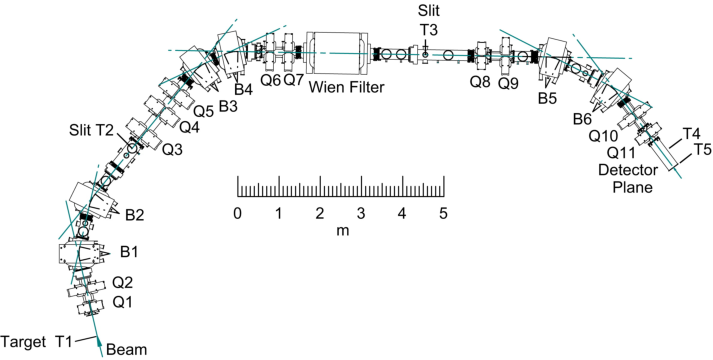
\includegraphics{stgeorge}
}
%\vspace{5cm}       % Give the correct figure height in cm
\caption{Schematic of the St. George recoil separator at the Institute for Nuclear Structure and Astrophysics, Notre Dame University (currently under construction). Taken from \cite{cou08}.}
\label{fig:stgeorge}
\end{center}
\end{figure*}



\subsection{Suggested avenues of technical development} 

With the pioneering measurements made of radiative capture in inverse kinematics over the last few decades, much has been learned and many techniques have been refined. With new recoil separators planned at radioactive beam or `rare isotope' facilities around the world, the proponents have a variety of solutions and methods at their disposal to enable very difficult measurements to take place. One factor that should be considered in the building of recoils separators is versatility. A separator like DRAGON, for example, was built to study lower mass capture reactions with very intense radioactive beams of large emittance, and thus had to have extremely good beam suppression, but at the expense of geometric acceptance. This limited the number of feasible reactions somewhat (or rather simply required extensive simulation to determine efficiencies with a resulting increase in systematic uncertainties). However it has been shown that the separator, with minor modifications, could be used successfully for a program in high mass radiative reactions ($A>70$). Other separators may similarly find new avenues of performance that are beyond what was planned in the design stage. There are several areas in which the authors might suggest, based on their knowledge of past performance of recoil separators, that improvements can be made to ensure versatility.

\subsubsection{Acceptance}

\subsubsection{Rigidity}

Rigidity is often a defining parameter of a recoil separator as magnetic and electrostatic elements come with inherent maximum operable field strengths. However, upgrading a separator to operate beyond its maximum design rigidity is only a technical matter. Magnetic elements are limited usually only by the capacity of the corresponding power supplies, the ability to cool the supplies and the magnets, and the ability to measure the magnetic fields precisely enough for your purposes over a wide enough energy range. 

For example, a magnetic dipole in a MEME design like DRAGON is essential for determination of the beam energy, and thus requires precise $\vec{B}$ measurement, usually using a nuclear magnetic resonance probe.  Such probes tend to have certain operable ranges with a minimum and maximum field strength. For a typical recoil separator interested in low energy reactions typical of stellar and nova scenarios, a single probe may be able to span a range of around 0.1-0.6 tesla, enough for a wide variety of available light-mass recoil charge states and momenta. However, for high mass reactions it gets more difficult to equilibrate in very high charge states, even with charge state boosting devices installed after the gas target. This means the rigidity requirements become more stringent, and it would be beneficial to be able to operate with much higher fields. In that case, consideration could be given to being able to switch between two installed NMR probes for operation in low and high field ranges, and to provide the capability of a cooling boost for the power supplies when operating in the high field region.   

In MEME designs the electric field becomes the limit as one goes to higher charge states as was seen in figure \ref{rigidity}. In that case it is the conditioning ability and the power supply capability that limits going to higher field strengths. Although the electric dipoles at the DRAGON facility have only been able to go as high as $\pm230$ kV because of conditioning issues, new designs like the EMMA dipoles will be able to reach as much as $\pm300$ kV over a 12.5 cm gap \cite{dav05} leading to a maximum field gradient of 5 MV/m compared to to DRAGON's 4.6 MV/m, and a maximum rigidity of 25 MV due to the larger bending radius. Consideration should be given in separator design to the advantages/disadvantages of larger radii/rigidity electric devices, and other more logistical requirements such as the available floor space in an experimental area may come into play when doing this, an issue that also affects Wien filters due to the need for internal or external power supplies. 
 
\subsubsection{Operation}

\subsubsection{Detection}